\documentclass[a4paper,14pt]{article}

\usepackage{pgfpages}

\usepackage[T2A]{fontenc}
\usepackage[utf8]{inputenc}
\usepackage[russian]{babel}

\usepackage{physics}
\usepackage{amsthm, amsmath, amssymb}
\usepackage{mathtext}
\usepackage[makeroom]{cancel}

% biber recommends this
\usepackage{csquotes}

\usepackage[
    colorlinks=true,
    linkcolor=black,
    anchorcolor=black,
    citecolor=black,
    filecolor=black,
    menucolor=black,
    runcolor=black,
    urlcolor=black
]{hyperref}
\usepackage[backend=biber,citestyle=numeric]{biblatex}
\addbibresource{~/data/references.bib}

\usepackage{graphicx}
\usepackage{graphbox}
\graphicspath{ {./images/} }

\linespread{1.5}
\setlength{\parindent}{1.25cm}

\usepackage{geometry}
\geometry{left=3cm}
\geometry{right=1.5cm}
\geometry{top=2cm}
\geometry{bottom=2cm}

% \newtheorem{theorem}{Теорема}
% \newtheorem{proposition}{Утверждение}
% \newtheorem{lemma}{Лемма}

% \theoremstyle{definition}
% \newtheorem{definition}{Определение}


\title{Оценка перерегулирования дифференциально-разностных управляемых систем}
\author{Шаршуков Владислав}
\date{2023}

\begin{document}

\begin{titlepage}
  \begin{center}
    САНКТ-ПЕТЕРБУРГСКИЙ ГОСУДАРСТВЕННЫЙ УНИВЕРСИТЕТ \\
    Направление: 01.03.02 «Прикладная математика и информатика» \\
    ООП: Прикладная математика, фундаментальная информатика и программирование \\[4cm]

    \textbf{ОТЧЕТ О НАУЧНО-ИССЛЕДОВАТЕЛЬСКОЙ РАБОТЕ}\\
  \end{center}
  \textbf{Тема задания:} Оценка перерегулирования
  дифференциально-разностных управляемых систем \\[0.5cm]
  \textbf{Выполнил:} Шаршуков Владислав \qquad 20.Б04-пу \\ [1.5cm]
  \textbf{Руководитель практики:} \\Жабко Алексей Петрович,
  доктор физ.-мат. наук, профессор, заведующий кафедрой теории
  управления
  \vspace{5cm}
  \begin{center}
    Санкт-Петербург\\
    2023
  \end{center}
\end{titlepage}

\setcounter{page}{2}

\begin{center}
  \tableofcontents
\end{center}

\newpage

\section{Введение}

\section{Обзор литературы}

Разные подходы: через решение матричных неравенств~\cite{modie2005},
через оценки функционала полного типа~\cite{kharitonov2013, kharitonov2004},

В настоящей работе рассматривается скалярное уравнение с постоянным
запаздыванием, для которого вариационными методами будет получена
точная оценка функционала полного типа.

\section{Постановка задачи}
Рассмотрим скалярное дифференциальное уравнение с запаздыванием:
\begin{equation}
  \label{eq:main-system}
  \dot x(t) = a_0 x(t) + a_1 x(t - h),
  \qquad h = \mathrm{const} > 0,
  \quad a_1 \neq 0.
\end{equation}
Будем считать систему~\eqref{eq:main-system} экспоненциально устойчивой.
В этом случае справедливо~\cite[стр.~66]{kharitonov2013}, что если
$U(\tau)$ --- матрица Ляпунова для матрицы $W = W_0 + W_1 + W_2 h$, причём
$W_0, W_1, W_2 > 0$, то функционал полного типа
\begin{equation*}
  \begin{aligned}
    v(\varphi)
    &=
      U(0) \varphi^2(0)
      +
      2 a_1 \varphi(0) \int\limits_{-h}^{0} U(-h - \theta) \varphi(\theta) d\theta
      + \\
    &\phantom{=}
      +
      \int\limits_{-h}^{0} a_1^2 \varphi(\theta_1) \left[
      \int\limits_{-h}^{0} U(\theta_1 - \theta_2) \varphi(\theta_2) d\theta_2
      \right] d\theta_1
      + \\
    &\phantom{=}
      +
      \int\limits_{-h}^{0} \left[
      W_1 + (h + \theta) W_2
      \right] \varphi^2(\theta) d\theta
  \end{aligned}
\end{equation*}
допускает оценку
\begin{equation}
  \label{eq:estimate}
  \alpha_1 \norm{\varphi(0)}^2
  \leqslant
  v(\varphi)
  \leqslant
  \alpha_2 \norm{\varphi}_h^2,
  \qquad
  \varphi \in PC([-h, 0], \mathbb{R}),
\end{equation}
где $\alpha_1, \alpha_2 > 0$ --- некоторые константы. Решение исходной
системы~\eqref{eq:main-system} тогда~\cite[стр.~67]{kharitonov2013} допускает
оценку
\begin{equation*}
  \norm{x(t, \varphi)} \leqslant \gamma \norm{\varphi}_h e^{-\sigma t},
  \qquad t \geqslant 0,
\end{equation*}
где $\gamma = \sqrt{\dfrac{\alpha_2}{\alpha_1}}$.

Заметим, что $\alpha_1$ и $\alpha_2$ можно рассматривать как функции переменных
$W_0, W_1, W_2$, поэтому можно поставить оптимизационную задачу: найти
максимальное значение для $\alpha_1$ и минимальное значение для $\alpha_2$, при
которых оценка~\eqref{eq:estimate} справедлива.

\section{Результат}

Известно~\cite[стр.~51]{kharitonov2013}, что если система~\eqref{eq:main-system}
удовлетворяет условию Ляпунова, т.е. если спектр этой системы
\begin{equation*}
  \Lambda = \left\{ s \in \mathbb{C}: s - a_0 - e^{-sh} a_1 = 0 \right\}
\end{equation*}
не содержит ни одного корня $s_0$ такого, чтобы и $-s_0$ принадлежал спектру
$\Lambda$, то для любой симметричной матрицы $W$ существует единственная матрица
Ляпунова $U(\tau)$. Очевидно, для любой экспоненциально устойчивой системы
условие Ляпунова выполняется. Для нахождения матрицы Ляпунова достаточно решить
вспомогательную систему уравнений
\begin{equation}
  \label{eq:aux-system}
  \begin{aligned}
    \frac{d }{d \tau} Y(\tau) &= \phantom{-}a_0 Y(\tau) + a_1 Z(\tau), \\
    \frac{d }{d \tau} Z(\tau) &= -a_1 Y(\tau) - a_0 Z(\tau)
  \end{aligned}
\end{equation}
с граничными условиями
\begin{equation}
  \label{eq:aux-boundaries}
  Y(0) = Z(h),
  \qquad
  2 a_0 Y(0) + a_1 Y(h) + a_1 Z(0) = -W.
\end{equation}

Для её решения сведём её к одному дифференциальному уравнению:
\begin{equation*}
  \begin{aligned}
    \frac{d^2 Y}{d \tau^2}
    &=
      a_0 \frac{d Y}{d \tau} + a_1 \frac{d Z}{d \tau} = \\
    &=
      a_0 \frac{d Y}{d \tau} - a_1^2 Y - a_0 a_1 Z.
  \end{aligned}
\end{equation*}
Из первого уравнения~\eqref{eq:aux-system} следует, что
\begin{equation*}
  Z = \frac{1}{a_1} \frac{d Y}{d \tau} - \frac{a_0}{a_1} Y,
\end{equation*}
поэтому
\begin{equation}
  \label{eq:aux-eq}
  \begin{aligned}
    \frac{d^2 Y}{d \tau^2}
    &= \cancel{a_0 \frac{d Y}{d \tau}} - a_1^2 Y
      - \cancel{a_0 \frac{d Y}{d \tau}} + a_0^2 Y = \\
    &= \left( a_0^2 - a_1^2 \right) Y.
  \end{aligned}
\end{equation}
Получили обыкновенное дифференциальное уравнение 2-го порядка. Его
характеристическое уравнение:
\begin{equation}
  \label{eq:aux-char}
  \lambda^2 = a_0^2 - a_1^2.
\end{equation}
Его корни зависят от знака правой части, поэтому рассмотрим три
возможных варианта.

\subsection{Случай $a_0^2 = a_1^2$}

В этом случае характеристическое уравнение~\eqref{eq:aux-char}
имеет один вещественный корень
\begin{equation*}
  \lambda = 0.
\end{equation*}
Решение исходного уравнения~\eqref{eq:aux-eq} представляется в
виде
\begin{equation*}
  Y = C_1 \tau + C_2.
\end{equation*}
Выразим теперь $Z(\tau)$ через $Y(\tau)$:
\begin{equation*}
  \begin{aligned}
    Z
    &=
      \frac{1}{a_1} \frac{d Y}{d \tau} - \frac{a_0}{a_1} Y = \\
    &=
      \frac{1}{a_1} C_1
      - \frac{a_0}{a_1} \left(
      C_1 \tau + C_2
      \right) = \\
    &=
      - \frac{a_0}{a_1} C_1 \tau
      + \frac{C_1 - a_0 C_2}{a_1}.
  \end{aligned}
\end{equation*}
Итак, решение вспомогательной системы~\eqref{eq:aux-system}
имеет вид
\begin{equation}
  \begin{aligned}
    Y &= C_1 \tau + C_2, \\
    Z &=
        - \frac{a_0}{a_1} C_1 \tau
        + \frac{C_1 - a_0 C_2}{a_1}.
  \end{aligned}
\end{equation}

Удовлетворим теперь граничным условиям~\eqref{eq:aux-boundaries}.
Подставим в них полученные представления для $Y$ и $Z$. Из
первого условия $Y(0) = Z(h)$ следует, что
\begin{equation*}
  C_2 =
  - \frac{a_0}{a_1} C_1 h
  + \frac{C_1 - a_0 C_2}{a_1}.
\end{equation*}
Из второго $2 a_0 Y(0) + a_1 Y(h) + a_1 Z(0) = -W$:
\begin{equation*}
  2 a_0 C_2 + a_1 (C_1 h + C_2) + C_1 - a_0 C_2 = -W.
\end{equation*}
После упрощений приходим к следующей системе уравнений:
\begin{equation*}
  \begin{aligned}
    \left(
    \frac{a_0}{a_1} h - \frac{1}{a_1}
    \right) C_1
    + \left(
    \frac{a_0}{a_1} + 1
    \right) C_2 &= 0, \\
    (a_1 h + 1) C_1 + (a_0 + a_1) C_2 &= -W.
  \end{aligned}
\end{equation*}
Найдём её определитель:
\begin{equation*}
  \begin{aligned}
    \Delta
    &=
      \left(
      \frac{a_0}{a_1} h - \frac{1}{a_1}
      \right)
      (a_0 + a_1)
      -
      \left(
      \frac{a_0}{a_1} + 1
      \right)
      (a_1 h + 1) = \\
    &=
      \frac{h a_0^2}{a_1} - h a_1
      - \frac{2 a_0}{a_1} - 2
  \end{aligned}
\end{equation*}
Так как $a_0^2 = a_1^2$, то
\begin{equation*}
  \begin{aligned}
    \Delta
    &=
      \frac{h a_1^2}{a_1} - h a_1
      - \frac{2 a_0}{a_1} - 2 = \\
    &=
      h a_1 - h a_1 - \frac{2 a_0}{a_1} - 2 = \\
    &=
      - 2 \left(
      \frac{a_0}{a_1} + 1
      \right).
  \end{aligned}
\end{equation*}
Из условия экспоненциальной устойчивости системы~\eqref{eq:main-system} следует,
что условию $a_0^2 = a_1^2$ удовлетворяет множество $a_0 = a_1$ при условии
$a_0 < 0$ (см. $D$-разбиение в~\cite[стр.~126]{elsgolc1971}
и~\autoref{fig:first-case}). Отсюда следует, что
\begin{equation*}
  \Delta
  =
  - 2 \left(
    \frac{a_0}{a_1} + 1
  \right)
  =
  -2 \cdot 2 = -4 \neq 0.
\end{equation*}

\begin{figure}
  \centering
  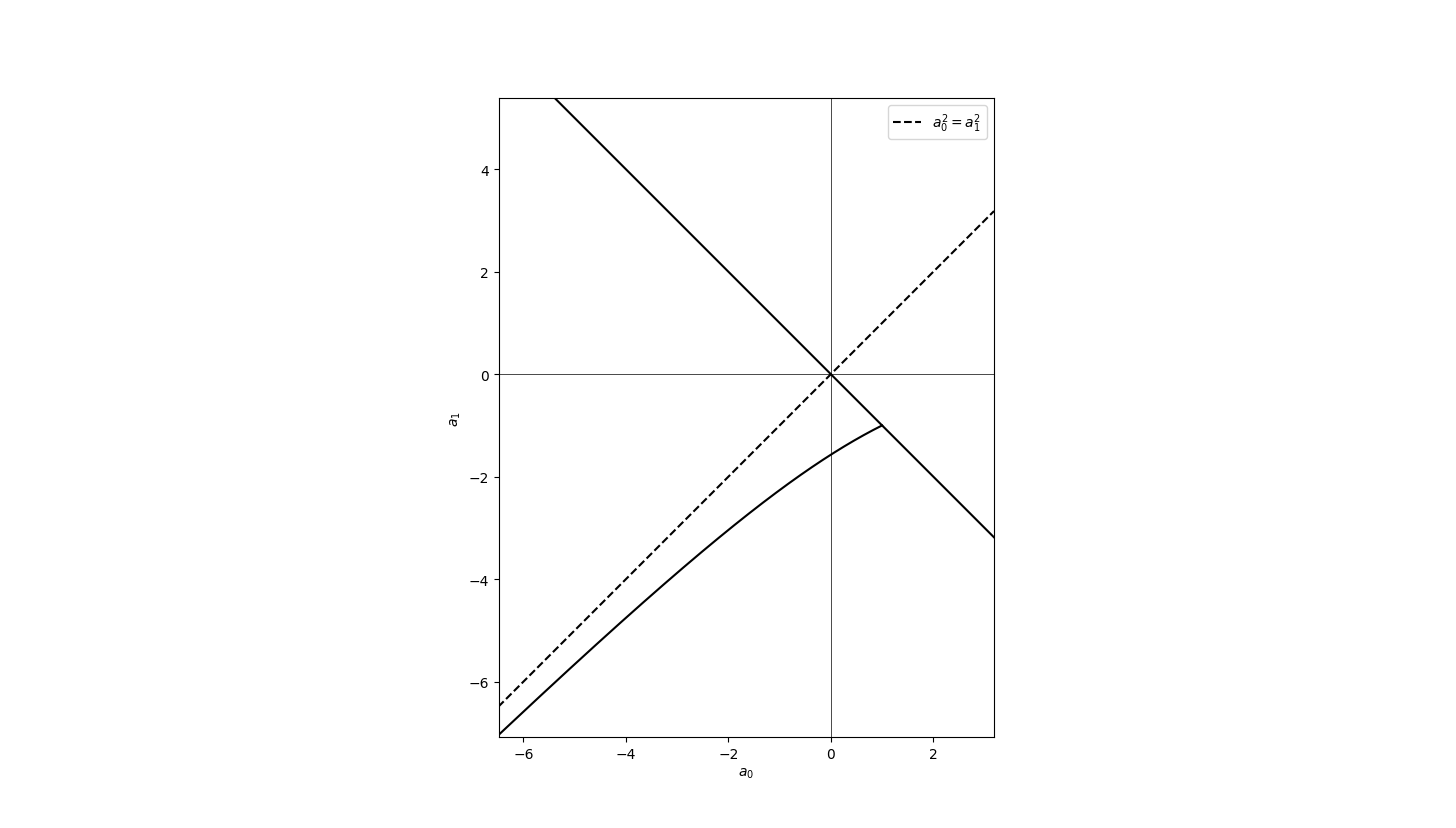
\includegraphics[width=\textwidth]{first-case}
  \caption{Граница $D$-разбиения}\label{fig:first-case}
\end{figure}

Так как матрица невырожденная, то константы $C_1, C_2$
определяются однозначно:
\begin{equation*}
  \begin{aligned}
    C_1
    &=
      \frac{\Delta_1}{\Delta}
      =
      -\frac{1}{4}
      \begin{vmatrix}
        0 & \dfrac{a_0}{a_1} + 1 \\
        -W & a_0 + a_1
      \end{vmatrix}
      =
      - \frac{W}{2}, \\
    C_2
    &=
      \frac{\Delta_2}{\Delta}
      =
      - \frac{1}{4}
      \begin{vmatrix}
        h - \dfrac{1}{a_1} & 0 \\
        a_1 h + 1 & -W
      \end{vmatrix}
      =
      \frac{a_1 h - 1}{4 a_1} W.
  \end{aligned}
\end{equation*}
Значит, решение вспомогательной системы равно
\begin{equation*}
  \begin{aligned}
    Y(\tau)
    &=
      -\frac{W}{2} \tau + \frac{a_1 h - 1}{4 a_1} W, \\
    Z(\tau)
    &=
      \frac{W}{2} \tau
      - \frac{W}{2 a_1}
      - \frac{a_1 h - 1}{4 a_1} W = \\
    &=
      \frac{W}{2} \tau
      - \frac{a_1 h + 1}{4 a_1} W.
  \end{aligned}
\end{equation*}

Так как константы $C_1, C_2$ определяются однозначно, то матрица
Ляпунова принимает вид~\cite[стр.~49]{kharitonov2013}
\begin{equation*}
  U(\tau) = Y(\tau)
  = - \frac{W}{2} \tau + \frac{a_1 h - 1}{4 a_1} W,
  \qquad \tau \in [0, h].
\end{equation*}

\subsubsection{Минимизация функционала полного типа}
Построим функционал полного типа, следуя~\cite{kharitonov2013}.  В
рассматриваемом случае
\begin{equation*}
  \begin{aligned}
    v_0(\varphi)
    &=
      \frac{a_1 h - 1}{4 a_1} \varphi^2(0)
      + 2 \varphi(0)
      \int\limits_{-h}^0 \left(
      \frac{W}{2} (h + \theta) + \frac{a_1 h - 1}{4a_1} W
      \right) a_1 \varphi(\theta) d\theta + \\
    &\phantom{=}
      + \int\limits_{-h}^0 \varphi(\theta_1) a_1 \left[
      \int\limits_{-h}^0 \left(
      \frac{W}{2} (\theta_2 - \theta_1)
      + \frac{a_1 h - 1}{4 a_1} W
      \right) a_1 \varphi(\theta_2) d\theta_2
      \right] d\theta_1
  \end{aligned}
\end{equation*}
Тогда функционал полного типа имеет вид
\begin{equation*}
  \begin{aligned}
    v(\varphi)
    &=
      v_0(\varphi)
      +
      \int\limits_{-h}^0 \left[
      W_1 + (h + \theta) W_2
      \right] \varphi^2(\theta) d\theta.
  \end{aligned}
\end{equation*}
Введём обозначения:
\begin{equation*}
  \begin{aligned}
    P_1(\varphi)
    &=
      \int\limits_{-h}^0 \left(
      \frac{a_1 W}{2} (h + \theta) + \frac{a_1 h - 1}{4} W
      \right) \varphi(\theta) d\theta, \\
    P_2(\varphi)
    &=
      \int\limits_{-h}^0 \varphi(\theta_1) \left[
      \int\limits_{-h}^0 \left(
      \frac{a_1 W}{2} (\theta_2 - \theta_1)
      + \frac{a_1 h - 1}{4} W
      \right) \varphi(\theta_2) d\theta_2
      \right] d\theta_1.
  \end{aligned}
\end{equation*}
Упростим эти слагаемые:
\begin{equation*}
  \begin{aligned}
    P_1(\varphi)
    &=
      \frac{a_1 W h}{2}
      \int\limits_{-h}^{0} \varphi(\theta) d\theta
      +
      \frac{a_1 W}{2}
      \int\limits_{-h}^{0} \theta \varphi(\theta) d\theta
      +
      \frac{a_1 h - 1}{4} W
      \int\limits_{-h}^{0} \varphi(\theta) d\theta = \\
    &=
      \left(
      \frac{a_1 W h}{2}
      +
      \frac{a_1 h - 1}{4} W
      \right)
      \int\limits_{-h}^{0} \varphi(\theta) d\theta
      +
      \frac{a_1 W}{2}
      \int\limits_{-h}^{0} \theta \varphi(\theta) d\theta = \\
    &=
      \frac{3 a_1 h - 1}{4}
      W
      \int\limits_{-h}^{0} \varphi(\theta) d\theta
      +
      \frac{a_1 W}{2}
      \int\limits_{-h}^{0} \theta \varphi(\theta) d\theta, \\
    P_2(\varphi)
    &=
      \int\limits_{-h}^{0} \varphi(\theta_1) \left[
      \frac{a_1 W}{2}
      \int\limits_{-h}^{0} \theta_2 \varphi(\theta_2) d\theta_2
      - \frac{a_1 W \theta_1}{2}
      \int\limits_{-h}^{0} \varphi(\theta_2) d\theta_2
      + \frac{a_1 h - 1}{4} W
      \int\limits_{-h}^{0} \varphi(\theta_2) d\theta_2
      \right] d\theta_1 = \\
    &=
      \cancel{
      \frac{a_1 W}{2}
      \int\limits_{-h}^{0} \varphi(\theta_1) d\theta_1
      \int\limits_{-h}^{0} \theta_2 \varphi(\theta_2) d\theta_2
      }
      -
      \cancel{
      \frac{a_1 W}{2}
      \int\limits_{-h}^{0} \theta_1 \varphi(\theta_1) d\theta_1
      \int\limits_{-h}^{0} \varphi(\theta_2) d\theta_2
      } + \\
    &\phantom{=}
      + \frac{a_1 h - 1}{4} W
      \int\limits_{-h}^{0} \varphi(\theta_1) d\theta_1
      \int\limits_{-h}^{0} \varphi(\theta_2) d\theta_2 = \\
    &=
      \frac{a_1 h - 1}{4} W
      \int\limits_{-h}^{0} \varphi(\theta_1) d\theta_1
      \int\limits_{-h}^{0} \varphi(\theta_2) d\theta_2.
  \end{aligned}
\end{equation*}
Итак, функционал полного типа будет иметь вид
\begin{equation*}
  \begin{aligned}
    v(\varphi)
    &=
      \frac{a_1 h - 1}{4 a_1} \varphi^2(0)
      +
      \frac{3 a_1 h - 1}{2}
      W
      \varphi(0)
      \int\limits_{-h}^{0} \varphi(\theta) d\theta
      +
      a_1 W \varphi(0)
      \int\limits_{-h}^{0} \theta \varphi(\theta) d\theta + \\
    &\phantom{=}
      +
      \frac{a_1^2 h - a_1}{4} W
      {\left(
      \int\limits_{-h}^{0} \varphi(\theta) d\theta
      \right)}^2
      +
      \left( W_1 + h W_2 \right)
      \int\limits_{-h}^{0} \varphi^2(\theta) d\theta
      +
      W_2
      \int\limits_{-h}^{0} \theta \varphi^2(\theta) d\theta.
  \end{aligned}
\end{equation*}

Перепишем нижнюю оценку~\eqref{eq:estimate} в виде
\begin{equation*}
  v(\varphi) - \alpha_1 \varphi^2(0) \geqslant 0.
\end{equation*}
Найдём минимум функционала на множестве непрерывных
на отрезке $[-h, 0]$ функций:
\begin{equation*}
  \begin{aligned}
    g(\varphi)
    &:=
      v(\varphi) - \alpha_1 \varphi^2(0) = \\
    &=
      \left(
      \frac{a_1 h - 1}{4 a_1}
      - \alpha_1
      \right)
      \varphi^2(0)
      +
      \frac{3 a_1 h - 1}{2}
      W
      \varphi(0)
      \int\limits_{-h}^{0} \varphi(\theta) d\theta
      +
      a_1 W \varphi(0)
      \int\limits_{-h}^{0} \theta \varphi(\theta) d\theta + \\
    &\phantom{=}
      +
      \frac{a_1^2 h - a_1}{4} W
      {\left(
      \int\limits_{-h}^{0} \varphi(\theta) d\theta
      \right)}^2
      +
      \left( W_1 + h W_2 \right)
      \int\limits_{-h}^{0} \varphi^2(\theta) d\theta
      +
      W_2
      \int\limits_{-h}^{0} \theta \varphi^2(\theta) d\theta.
  \end{aligned}
\end{equation*}
Заметим, что тривиальная начальная функция $\varphi \equiv 0$
нас не интересует, так как для неё оценки~\eqref{eq:estimate} справедливы
при всех $\alpha_1, \alpha_2$.

Необходимое условие слабого минимума функционала --- равенство нулю первой
вариации~\cite[стр.~289]{elsgolc1969}:
\begin{equation*}
  \delta g(\varphi(t))
  =
  {\left.
    \frac{\partial }{\partial \alpha} g(\varphi(t) + \alpha \delta \varphi)
  \right|}_{\alpha = 0} = 0.
\end{equation*}
Так как
\begin{equation*}
  \begin{aligned}
    g(\varphi(t) + \alpha \delta \varphi)
    &=
      \left(
      \frac{a_1 h - 1}{4 a_1}
      - \alpha_1
      \right)
      {\left(
      \varphi(0) + \alpha \delta \varphi(0)
      \right)}^2
      +
      \frac{3 a_1 h - 1}{2}
      W
      \left( \varphi(0) + \alpha \delta \varphi(0) \right)
      \int\limits_{-h}^{0} \left(
      \varphi(\theta) + \alpha \delta \varphi
      \right) d\theta + \\
    &\phantom{=}
      +
      a_1 W \left( \varphi(0) + \alpha \delta \varphi(0) \right)
      \int\limits_{-h}^{0} \theta \left(
      \varphi(\theta) + \alpha \delta \varphi
      \right)d\theta
      +
      \frac{a_1^2 h - a_1}{4} W
      {\left(
      \int\limits_{-h}^{0} \left(
      \varphi(\theta) + \alpha \delta \varphi
      \right) d\theta
      \right)}^2 + \\
    &\phantom{=}
      +
      \left( W_1 + h W_2 \right)
      \int\limits_{-h}^{0} {\left(
      \varphi(\theta) + \alpha \delta \varphi
      \right)}^2 d\theta
      +
      W_2
      \int\limits_{-h}^{0} \theta {\left(
      \varphi(\theta) + \alpha \delta \varphi
      \right)}^2 d\theta,
  \end{aligned}
\end{equation*}
то
\begin{equation}
  \label{eq:first-pd}
  \begin{aligned}
    \frac{\partial }{\partial \alpha}
    g(\varphi(t) + \alpha \delta \varphi)
    &=
      \left(
      \frac{a_1 h - 1}{2 a_1}
      - 2 \alpha_1
      \right)
      \left(
      \varphi(0) + \alpha \delta \varphi(0)
      \right)
      \delta \varphi(0)
      +
      \frac{3 a_1 h - 1}{2}
      W
      \delta \varphi(0)
      \int\limits_{-h}^{0} \left(
      \varphi(\theta) + \alpha \delta \varphi
      \right) d\theta + \\
    &\phantom{=}
      +
      \frac{3 a_1 h - 1}{2}
      W
      \left( \varphi(0) + \alpha \delta \varphi(0) \right)
      \int\limits_{-h}^{0} \delta \varphi d\theta
      +
      a_1 W \delta \varphi(0)
      \int\limits_{-h}^{0} \theta \left(
      \varphi(\theta) + \alpha \delta \varphi
      \right)d\theta + \\
    &\phantom{=}
      +
      a_1 W \left( \varphi(0) + \alpha \delta \varphi(0) \right)
      \int\limits_{-h}^{0} \theta \delta \varphi d\theta
      +
      \frac{a_1^2 h - a_1}{2} W
      \left(
      \int\limits_{-h}^{0} \left(
      \varphi(\theta) + \alpha \delta \varphi
      \right) d\theta
      \right)
      \int\limits_{-h}^{0} \delta \varphi d\theta
      + \\
    &\phantom{=}
      +
      2 \left( W_1 + h W_2 \right)
      \int\limits_{-h}^{0} \left(
      \varphi(\theta) + \alpha \delta \varphi
      \right) \delta \varphi d\theta
      +
      2 W_2
      \int\limits_{-h}^{0} \theta \left(
      \varphi(\theta) + \alpha \delta \varphi
      \right) \delta \varphi d\theta.
  \end{aligned}
\end{equation}
Окончательно имеем
\begin{equation*}
  \begin{aligned}
    \delta g(\varphi(t))
    &=
      {\left.
      \frac{\partial }{\partial \alpha} g(\varphi(t) + \alpha \delta \varphi)
      \right|}_{\alpha = 0} = \\
    &=
      \left(
      \frac{a_1 h - 1}{2 a_1}
      - 2 \alpha_1
      \right)
      \varphi(0)
      \delta \varphi(0)
      +
      \frac{3 a_1 h - 1}{2}
      W
      \delta \varphi(0)
      \int\limits_{-h}^{0} \varphi(\theta) d\theta + \\
    &\phantom{=}
      +
      \frac{3 a_1 h - 1}{2}
      W
      \varphi(0)
      \int\limits_{-h}^{0} \delta \varphi d\theta
      +
      a_1 W \delta \varphi(0)
      \int\limits_{-h}^{0} \theta \varphi(\theta) d\theta + \\
    &\phantom{=}
      +
      a_1 W \varphi(0)
      \int\limits_{-h}^{0} \theta \delta \varphi d\theta
      +
      \frac{a_1^2 h - a_1}{2} W
      \int\limits_{-h}^{0} \varphi(\theta) d\theta
      \cdot
      \int\limits_{-h}^{0} \delta \varphi d\theta
      + \\
    &\phantom{=}
      +
      2 \left( W_1 + h W_2 \right)
      \int\limits_{-h}^{0} \varphi(\theta)
      \delta \varphi d\theta
      +
      2 W_2
      \int\limits_{-h}^{0} \theta \varphi(\theta)
      \delta \varphi d\theta = \\
    &=
      \left[
      \left(
      \frac{a_1 h - 1}{2 a_1}
      - 2 \alpha_1
      \right)
      \varphi(0)
      +
      \frac{3 a_1 h - 1}{2}
      W
      \int\limits_{-h}^{0} \varphi(\theta) d\theta
      +
      a_1 W
      \int\limits_{-h}^{0} \theta \varphi(\theta) d\theta
      \right] \delta \varphi(0)
      + \\
    &\phantom{=}
      \int\limits_{-h}^{0}
      \left[
      \frac{3 a_1 h - 1}{2}
      W
      \varphi(0)
      +
      a_1 W \varphi(0) \theta
      +
      \frac{a_1^2 h - a_1}{2} W
      \int\limits_{-h}^{0} \varphi(\theta) d\theta
      +
      \right. \\
    &\phantom{=}
      \left.
      \phantom{\int\limits_{-h}^{0}}
      +
      2 \left( W_1 + h W_2 \right)
      \varphi(\theta)
      +
      2 W_2
      \theta \varphi(\theta)
      \right] \delta \varphi d\theta = 0.
  \end{aligned}
\end{equation*}
Если $\delta \varphi(0) = 0$, то необходимое условие принимает вид
\begin{equation*}
  \begin{aligned}
    \delta g(\varphi)
    &=
      \int\limits_{-h}^{0}
      \left[
      \frac{3 a_1 h - 1}{2}
      W
      \varphi(0)
      +
      a_1 W \varphi(0) \theta
      +
      \frac{a_1^2 h - a_1}{2} W
      \int\limits_{-h}^{0} \varphi(\theta) d\theta
      +
      \right. \\
    &\phantom{=}
      \left.
      \phantom{\int\limits_{-h}^{0}}
      +
      2 \left( W_1 + h W_2 \right)
      \varphi(\theta)
      +
      2 W_2
      \theta \varphi(\theta)
      \right] \delta \varphi d\theta = 0.
  \end{aligned}
\end{equation*}
Из основной леммы вариационного исчисления~\cite[стр.~295]{elsgolc1969}
следует первое необходимое условие минимума функционала:
\begin{equation}
  \label{eq:necessity-1}
  \frac{3 a_1 h - 1}{2}
  W
  \varphi(0)
  +
  a_1 W \varphi(0) t
  +
  \frac{a_1^2 h - a_1}{2} W
  \int\limits_{-h}^{0} \varphi(\theta) d\theta
  +
  2 \left( W_1 + h W_2 \right)
  \varphi(t)
  +
  2 W_2
  t \varphi(t) = 0.
\end{equation}
Пусть теперь $\delta \varphi(0)$ произвольно. Тогда, учитывая необходимое
условие~\eqref{eq:necessity-1}, первая вариация принимает вид
\begin{equation*}
  \delta g(\varphi(t))
  =
  \left[
    \left(
      \frac{a_1 h - 1}{2 a_1}
      - 2 \alpha_1
    \right)
    \varphi(0)
    +
    \frac{3 a_1 h - 1}{2}
    W
    \int\limits_{-h}^{0} \varphi(\theta) d\theta
    +
    a_1 W
    \int\limits_{-h}^{0} \theta \varphi(\theta) d\theta
  \right] \delta \varphi(0) = 0.
\end{equation*}
Так как $\delta \varphi(0)$ --- произвольная внутренняя точка множества
значений функции $\varphi$, то получаем второе необходимое условие
минимума функционала:
\begin{equation}
  \label{eq:necessity-2}
  \left(
    \frac{a_1 h - 1}{2 a_1}
    - 2 \alpha_1
  \right)
  \varphi(0)
  +
  \frac{3 a_1 h - 1}{2}
  W
  \int\limits_{-h}^{0} \varphi(\theta) d\theta
  +
  a_1 W
  \int\limits_{-h}^{0} \theta \varphi(\theta) d\theta
  = 0.
\end{equation}
Итак, необходимые условия слабого экстремума для функционала
$g(\varphi)$ можно записать так:
\begin{equation}
  \label{eq:necessary-conds}
  \begin{aligned}
    \left[
    \frac{3 a_1 h - 1}{2}
    W
    +
    a_1 W t
    \right] \varphi(0)
    +
    \frac{a_1^2 h - a_1}{2} W
    \int\limits_{-h}^{0} \varphi(\theta) d\theta
    +
    2
    \left[
    W_1
    + W_2
    \left( h + t \right)
    \right]
    \varphi(t)
    &=
      0, \\
    \left(
    \frac{a_1 h - 1}{2 a_1}
    - 2 \alpha_1
    \right)
    \varphi(0)
    +
    \int\limits_{-h}^{0}
    \left[
    \frac{3 a_1 h - 1}{2}
    W
    +
    a_1 W \theta
    \right] \varphi(\theta) d\theta
    &=
      0.
  \end{aligned}
\end{equation}

\subsubsection{Вычисление экстремали}
Заметим, что первое из необходимых условий~\eqref{eq:necessary-conds} является
интегральным уравнением Фредгольма второго рода, а второе --- интегральным
уравнением Фредгольма первого рода. Их можно переписать в более привычном виде:
\begin{equation*}
  \begin{gathered}
    \varphi(t)
    =
    \int\limits_{-h}^{0}
      \frac{(a_1 - a_1^2 h) W}{4 (W_1 + W_2 (h + t))}
      \varphi(\theta) d\theta
    -
    \frac{W (3 a_1 h - 1 + 2 a_1 t)}{4 (W_1 + W_2 (h + t))}
    \varphi(0), \\
    \int\limits_{-h}^{0}
    \left[
      \frac{3 a_1 h - 1}{2}
      W
      +
      a_1 W \theta
    \right] \varphi(\theta) d\theta
    =
    \left(
      2 \alpha_1
      -
      \frac{a_1 h - 1}{2 a_1}
    \right)
    \varphi(0).
  \end{gathered}
\end{equation*}

Рассмотрим первое уравнение, считая, что $\varphi(0) = \varphi_0$:
\begin{equation}
  \label{eq:first-fredholm}
  \varphi(t) = \lambda \int\limits_{-h}^{0} K(t, \theta) \varphi(\theta) d\theta + f(t),
\end{equation}
где введены обозначения
\begin{equation*}
  \lambda = 1,
  \qquad
  K(t, \theta) = \frac{(a_1 - a_1^2 h) W}{4 (W_1 + W_2 (h + t))},
  \qquad
  f(t)
  = -\frac{W (3 a_1 h - 1 + 2 a_1 t)}{4 (W_1 + W_2 (h + t))} \varphi_0.
\end{equation*}
Ядро $K(t, \theta)$ является вырожденным~\cite[стр.~189]{bicadze1982}:
\begin{equation*}
  K(t, \theta) = \frac{(a_1 - a_1^2 h) W}{4 (W_1 + W_2 (h + t))} = p(t),
\end{equation*}
поэтому исходное уравнение можно переписать в виде
\begin{equation}
  \label{eq:first-fredholm-sol}
  \varphi(t) = f(t) + \lambda c p(t),
\end{equation}
где ${\displaystyle c = \int\limits_{-h}^{0} \varphi(\theta) d\theta}$ ---
неизвестная постоянная. Для определения этой постоянной подставим
представление~\eqref{eq:first-fredholm-sol} решения в исходное
уравнение~\eqref{eq:first-fredholm}, получаем
\begin{equation*}
  f(t) + \lambda c p(t)
  =
  \lambda \int\limits_{-h}^{0}
  p(t) \left[ f(\theta) + \lambda c p(\theta) \right] d\theta
  + f(t),
\end{equation*}
или
\begin{equation*}
  p(t) \left[
    c -
    \int\limits_{-h}^{0}
    \left[ f(\theta) + \lambda c p(\theta) \right] d\theta
  \right]
  = 0,
\end{equation*}
откуда, в силу того, что $p(t) \neq 0$, следует равенство
\begin{equation*}
  c -
  \int\limits_{-h}^{0}
  \left[ f(\theta) + \lambda c p(\theta) \right] d\theta
  = 0.
\end{equation*}
Путём простых преобразований приходим к уравнению
\begin{equation*}
  c \left(
  1 - \lambda \int\limits_{-h}^{0} p(\theta) d\theta
  \right)
  =
  \int\limits_{-h}^{0} f(\theta) d\theta.
\end{equation*}
Вычислим интеграл:
\begin{equation*}
  \begin{aligned}
    \int\limits_{-h}^{0} p(\theta) d\theta
    &=
      \int\limits_{-h}^{0} \frac{(a_1 - a_1^2 h) W}{4 (W_1 + W_2 (h + \theta))} d\theta = \\
    &=
      \frac{(a_1 - a_1^2 h) W}{4 W_2}
      \int\limits_{-h}^{0} \frac{1}{W_1 + W_2 (h + \theta)} d(W_1 + W_2 (h + \theta)) = \\
    &=
      \frac{(a_1 - a_1^2 h) W}{4 W_2}
      \ln \left[W_1 + W_2 (h + \theta)\right] \Big|_{-h}^{0} = \\
    &=
      \frac{(a_1 - a_1^2 h) W}{4 W_2}
      \left[ \ln (W_1 + W_2 h) - \ln W_1 \right] = \\
    &=
      \frac{(a_1 - a_1^2 h) W}{4 W_2}
      \ln \left( 1 + \frac{W_2}{W_1} h \right).
  \end{aligned}
\end{equation*}
Заметим, что он не равен единице: из предположений
\begin{equation*}
  W_0, W_1, W_2 > 0, \qquad h > 0
\end{equation*}
следует, что логарифм и знаменатель больше нуля. Так как мы рассматриваем
случай $a_0^2 = a_1^2$, то из экспоненциальной устойчивости уравнения~\eqref{eq:main-system}
следует, что $a_1 < 0$, поэтому числитель меньше нуля и, следовательно, всё это
выражение меньше нуля.

Это в свою очередь означает, что $\lambda = 1$ не является собственным числом
ядра $K(t, \theta)$, поэтому из первой теоремы Фредгольма~\cite[стр.~191]{bicadze1982}
следует, что $\varphi(t)$ определяется единственным образом для любой непрерывной
правой части $f(t)$. Нетрудно убедиться, что $f(t)$ является непрерывной функцией
на отрезке $[-h, 0]$.

Для нахождения константы $c$ вычислим интеграл
\begin{equation*}
  \begin{aligned}
    \int\limits_{-h}^{0} f(\theta) d\theta
    &=
      - \int\limits_{-h}^{0} \frac{W (3 a_1 h - 1 + 2 a_1 \theta)}{4 (W_1 + W_2 (h + \theta))} \varphi_0 d\theta
      =
      - \frac{\varphi_0 W}{4}
      \int\limits_{-h}^{0} \frac{(3 a_1 h - 1) + 2 a_1 \theta}{(W_1 + W_2 h) + W_2 \theta} d\theta.
  \end{aligned}
\end{equation*}
Так как
\begin{equation}
  \label{eq:int-formula}
  \begin{aligned}
    \int\limits_{-h}^{0} \frac{c_1 + d_1 \theta}{c_2 + d_2 \theta} d\theta
    &=
      \frac{c_1}{d_2} \int\limits_{-h}^{0} \frac{1}{c_2 + d_2 \theta} d(c_2 + d_2 \theta)
      +
      \frac{d_1}{d_2} \int\limits_{-h}^{0} \frac{c_2 + d_2 \theta - c_2}{c_2 + d_2 \theta} d\theta
      = \\
    &=
      \frac{c_1}{d_2} \ln \abs{c_2 + d_2 \theta} \Big|_{-h}^0
      +
      \frac{d_1}{d_2} \int\limits_{-h}^{0} d \theta
      -
      \frac{d_1 c_2}{d_2^2} \int\limits_{-h}^{0} \frac{1}{c_2 + d_2 \theta} d(c_2 + d_2 \theta)
      = \\
    &=
      \frac{c_1}{d_2} \left(
      \ln \abs{c_2} - \ln \abs{c_2 - d_2 h}
      \right)
      +
      \frac{d_1}{d_2} h
      -
      \frac{d_1 c_2}{d_2^2} \ln \abs{c_2 + d_2 \theta} \Big|_{-h}^0
      = \\
    &=
      \frac{c_1 d_2 - d_1 c_2}{d_2^2} \left(
      \ln \abs{c_2} - \ln \abs{c_2 - d_2 h}
      \right)
      +
      \frac{d_1}{d_2} h,
  \end{aligned}
\end{equation}
а в нашем случае
\begin{equation*}
  \begin{aligned}
    c_1
    &=
      3 a_1 h - 1, &
    d_1
    &=
      2 a_1, \\
    c_2
    &=
      W_1 + W_2 h,
    &
    d_2
    &=
      W_2,
  \end{aligned}
\end{equation*}
поэтому
\begin{equation*}
  \begin{aligned}
    \int\limits_{-h}^{0} f(\theta) d\theta
    &=
      - \frac{\varphi_0 W}{4} \left[
      \frac{(3 a_1 h - 1) W_2 - 2 a_1 (W_1 + W_2 h)}{W_2^2} \left(
      \ln \left( W_1 + W_2 h \right)
      -
      \ln \left( W_1 + W_2 h - W_2 h \right)
      \right)
      +
      \frac{2 a_1}{W_2} h
      \right] = \\
    &=
      - \frac{\varphi_0 W}{4 W_2} \left[
      \frac{a_1 h W_2 - 2 a_1 W_1 - W_2}{W_2}
      \ln \left( 1 +  \frac{W_2}{W_1} h \right)
      +
      2 a_1 h
      \right].
  \end{aligned}
\end{equation*}
Итак, окончательно можно записать выражение для константы $c$:
\begin{equation*}
  \begin{aligned}
    c
    &=
      - \frac{\varphi_0 W}{4 W_2} \left[
      \frac{a_1 h W_2 - 2 a_1 W_1 - W_2}{W_2}
      \ln \left( 1 +  \frac{W_2}{W_1} h \right)
      +
      2 a_1 h
      \right]
      \cdot {\left[
      1 -
      \frac{(a_1 - a_1^2 h) W}{4 W_2}
      \ln \left( 1 + \frac{W_2}{W_1} h \right)
      \right]}^{-1}
      = \\
    &=
      - \frac{\varphi_0 W}{\cancel{4 W_2}} \left[
      \frac{a_1 h W_2 - 2 a_1 W_1 - W_2}{W_2}
      \ln \left( 1 +  \frac{W_2}{W_1} h \right)
      +
      2 a_1 h
      \right]
      \cdot \left[
      \frac{\cancel{4 W_2}}{4 W_2 - (a_1 - a_1^2 h) W
      \ln \left( 1 + \frac{W_2}{W_1} h \right)
      }
      \right]
      = \\
    &=
      - \varphi_0 W \cdot
      \frac{
      \left(a_1 h W_2 - 2 a_1 W_1 - W_2 \right)
      \ln \left( 1 +  \frac{W_2}{W_1} h \right)
      + 2 a_1 W_2 h
      }{W_2}
      \cdot
      \frac{1}{4 W_2 - (a_1 - a_1^2 h) W
      \ln \left( 1 + \frac{W_2}{W_1} h \right)
      }
      = \\
    &=
      - \frac{\varphi_0 W}{W_2}
      \cdot
      \frac{
      \left(a_1 h W_2 - 2 a_1 W_1 - W_2 \right)
      \ln \left( 1 +  \frac{W_2}{W_1} h \right)
      + 2 a_1 W_2 h
      }{4 W_2 - (a_1 - a_1^2 h) W
      \ln \left( 1 + \frac{W_2}{W_1} h \right)
      }.
  \end{aligned}
\end{equation*}
Тогда искомая функция $\varphi(t)$ записывается в виде
\begin{equation*}
  \begin{aligned}
    \varphi(t)
    &=
      -\frac{W (3 a_1 h - 1 + 2 a_1 t)}{4 (W_1 + W_2 (h + t))} \varphi_0
      - \frac{\varphi_0 W}{W_2}
      \cdot
      \frac{
      \left(a_1 h W_2 - 2 a_1 W_1 - W_2 \right)
      \ln \left( 1 +  \frac{W_2}{W_1} h \right)
      + 2 a_1 W_2 h
      }{4 W_2 - (a_1 - a_1^2 h) W
      \ln \left( 1 + \frac{W_2}{W_1} h \right)
      }
      \frac{(a_1 - a_1^2 h) W}{4 (W_1 + W_2 (h + t))}
      = \\
    &=
      - \frac{W \varphi_0}{4 (W_1 + W_2(h + t))}
      \left[
      2 a_1 t + 3 a_1 h - 1
      +
      \frac{
      \left(a_1 h W_2 - 2 a_1 W_1 - W_2 \right)
      \ln \left( 1 +  \frac{W_2}{W_1} h \right)
      + 2 a_1 W_2 h
      }{4 W_2 - (a_1 - a_1^2 h) W
      \ln \left( 1 + \frac{W_2}{W_1} h \right)
      }
      \frac{(a_1 - a_1^2 h) W}{W_2}
      \right].
  \end{aligned}
\end{equation*}
Для краткости будем представлять эту функцию в виде
\begin{equation*}
  \varphi(t) = - \frac{A t + B}{C t + D} \varphi_0,
\end{equation*}
где
\begin{equation*}
  \begin{aligned}
    A
    &=
      2 W a_1, \\
    B
    &=
      W
      \left[
      3 a_1 h - 1
      +
      \frac{
      \left(a_1 h W_2 - 2 a_1 W_1 - W_2 \right)
      \ln \left( 1 +  \frac{W_2}{W_1} h \right)
      + 2 a_1 W_2 h
      }{4 W_2 - (a_1 - a_1^2 h) W
      \ln \left( 1 + \frac{W_2}{W_1} h \right)
      }
      \frac{(a_1 - a_1^2 h) W}{W_2}
      \right], \\
    C
    &=
      4 W_2, \\
    D
    &=
      4 W_1 + 4 W_2 h.
  \end{aligned}
\end{equation*}
Проверим, что эта функция удовлетворяет второму необходимому
условию~\eqref{eq:necessary-conds}:
\begin{equation*}
    \int\limits_{-h}^{0}
    \left[
      \frac{3 a_1 h - 1}{2}
      W
      +
      a_1 W \theta
    \right] \varphi(\theta) d\theta
    =
    \left(
      2 \alpha_1
      -
      \frac{a_1 h - 1}{2 a_1}
    \right)
    \varphi(0).
\end{equation*}
Рассмотрим левую часть уравнения:
\begin{equation*}
  \begin{aligned}
    \int\limits_{-h}^{0}
    \left[
    \frac{3 a_1 h - 1}{2}
    W
    +
    a_1 W \theta
    \right] \varphi(\theta) d\theta
    &=
      - 2 \varphi_0
      \int\limits_{-h}^{0} \left(
      A \theta + B_1
      \right) \frac{A \theta + B_1 + B_2}{C \theta + D} d\theta = \\
    &=
      - 2 \varphi_0
      \left[
      \int\limits_{-h}^{0}
      \frac{{(A \theta + B_1)}^2}{C \theta + D} d\theta
      +
      B_2
      \int\limits_{-h}^{0}
      \frac{a \theta + b_1}{c \theta + d} d\theta
      \right],
  \end{aligned}
\end{equation*}
где
\begin{equation*}
  \begin{aligned}
    B_1 &= W (3 a_1 h - 1), \\
    B_2 &=
      \frac{
      \left(a_1 h W_2 - 2 a_1 W_1 - W_2 \right)
      \ln \left( 1 +  \frac{W_2}{W_1} h \right)
      + 2 a_1 W_2 h
      }{4 W_2 - (a_1 - a_1^2 h) W
      \ln \left( 1 + \frac{W_2}{W_1} h \right)
      }
      \frac{(a_1 - a_1^2 h) W^2}{W_2}.
  \end{aligned}
\end{equation*}

Рассмотрим первое слагаемое:
\begin{equation*}
  \begin{aligned}
    \int\limits_{-h}^{0} \frac{{(A \theta + B_1)}^2}{C \theta + D} d\theta
    &=
    \int\limits_{-h}^{0} \frac{A^2 \theta^2 + 2 A B_1 \theta + B_1^2}{C \theta + D} d\theta.
  \end{aligned}
\end{equation*}
Пусть $E := \dfrac{B_1}{A}$, тогда
\begin{equation*}
  \begin{aligned}
    \int\limits_{-h}^{0} \frac{A^2 \theta^2 + 2 A B_1 \theta + B_1^2}{C \theta + D} d\theta
    &=
      \frac{A^2}{C}
      \int\limits_{-h}^{0} \frac{C \theta^2 + 2 E C \theta + E^2 C}{C \theta + D} d\theta = \\
    &=
      \frac{A^2}{C}
      \int\limits_{-h}^{0} \frac{
      C \theta^2 + D \theta + (2 E C - D) \theta + E^2 C
      }{C \theta + D} d\theta = \\
    &=
      \frac{A^2}{C}
      \left[
      \int\limits_{-h}^{0} \theta d\theta
      +
      \int\limits_{-h}^{0} \frac{
      (2 E C - D) \theta + E^2 C
      }{C \theta + D} d\theta
      \right] \overset{\eqref{eq:int-formula}}{=} \\
    &=
      \frac{A^2}{C}
      \left[
      -
      \frac{h^2}{2}
      +
      \frac{E^2 C^2 - 2 E C D + D^2}{C^2}
      \ln \left( \frac{D}{D - C h} \right)
      +
      \frac{2 E C - D}{C} h
      \right] = \\
    &=
      -
      \frac{h^2 A^2}{2 C}
      +
      \frac{B_1^2 C^2 - 2 A B_1 C D + A^2 D^2}{C^3}
      \ln \left( \frac{D}{D - C h} \right)
      +
      \frac{2 A B_1 C - A^2 D}{C^2} h = \\
    &=
      -
      \frac{h^2 A^2}{2 C}
      +
      \frac{{(B_1 C - A D)}^2}{C^3}
      \ln \left( \frac{D}{D - C h} \right)
      +
      \frac{2 A B_1 C - A^2 D}{C^2} h.
  \end{aligned}
\end{equation*}
Для второго слагаемого можно сразу воспользоваться формулой~\eqref{eq:int-formula}:
\begin{equation*}
  \begin{aligned}
    \int\limits_{-h}^{0}
    \frac{A \theta + B_1}{C \theta + D} d\theta
    &=
      \frac{B_1 C - A D}{C^2}
      \ln \left( \frac{D}{D - C h} \right)
      +
      \frac{A}{C} h.
  \end{aligned}
\end{equation*}
Тогда
\begin{equation*}
  \begin{aligned}
    \int\limits_{-h}^{0}
    \left[
    \frac{3 a_1 h - 1}{2}
    W
    +
    a_1 W \theta
    \right] \varphi(\theta) d\theta
    &=
      -2 \varphi_0
      \left[
      -
      \frac{h^2 A^2}{2 C}
      +
      \frac{{(B_1 C - A D)}^2}{C^3}
      \ln \left( \frac{D}{D - C h} \right)
      +
      \frac{2 A B_1 C - A^2 D}{C^2} h
      \right. + \\
    &\phantom{= -2 \varphi_0}
      \left.
      + B_2 \left(
      \frac{B_1 C - A D}{C^2}
      \ln \left( \frac{D}{D - C h} \right)
      +
      \frac{A}{C} h
      \right)
      \right] = \\
    &=
      \varphi_0
      \left[
      \frac{h^2 A^2}{C}
      - 2
      \frac{B_1 C - A D}{C} \cdot
      \frac{B_1 C - A D}{C^2}
      \ln \left( \frac{D}{D - C h} \right)
      \right. - \\
    &\phantom{= -2 \varphi_0}
      \left.
      - 2 \frac{2 B_1 C - A D}{C} \cdot \frac{A}{C} h
      - 2 B_2
      \frac{B_1 C - A D}{C^2}
      \ln \left( \frac{D}{D - C h} \right)
      -2 B_2
      \frac{A}{C} h
      \right] = \\
    &=
      - 2
      \varphi_0
      \left[
      \left(
      B_2 + \frac{B_1 C - A D}{C}
      \right)
      \frac{B_1 C - A D}{C^2}
      \ln \left( \frac{D}{D - C h} \right)
      \right. + \\
    &\phantom{= -2 \varphi_0}
      \left.
      \left( B_2 + \frac{2 B_1 C - A D}{C} - \frac{A h }{2} \right)
      \frac{A}{C} h
      \right] = \\
    &=
      - 2
      \varphi_0
      \left[
      \frac{B C - A D}{C} \cdot
      \frac{B_1 C - A D}{C^2}
      \ln \left( \frac{D}{D - C h} \right)
      \right. + \\
    &\phantom{= -2 \varphi_0}
      \left.
      \left( \frac{B C + B_1 C - A D}{C} - \frac{A h }{2} \right)
      \frac{A}{C} h
      \right].
  \end{aligned}
\end{equation*}
Сравнивая полученное выражение с правой частью исходного уравнения
\begin{equation*}
  \left(
    2 \alpha_1
    -
    \frac{a_1 h - 1}{2 a_1}
  \right)
  \varphi(0)
  =
  -
  \left(
    2 \alpha_1
    -
    \frac{B_1 - A h}{A}
  \right)
  \frac{B}{D} \varphi_0,
\end{equation*}
приходим к выводу, что
\begin{equation*}
  \frac{B C - A D}{C} \cdot
  \frac{B_1 C - A D}{C^2}
  \ln \left( \frac{D}{D - C h} \right)
  +
  \left( \frac{B C + B_1 C - A D}{C} - \frac{A h }{2} \right)
  \frac{A}{C} h
  =
  \left(
    \alpha_1
    -
    \frac{B_1 - A h}{2 A}
  \right)
  \frac{B}{D}.
\end{equation*}
Значит, функция $\varphi(t)$ является единственной нетривиальной экстремалью
тогда и только тогда, когда
\begin{equation*}
  \alpha_1
  =
  \frac{D}{B} \cdot
  \frac{B C - A D}{C} \cdot
  \frac{B_1 C - A D}{C^2}
  \ln \left( \frac{D}{D - C h} \right)
  +
  \left( \frac{B C + B_1 C - A D}{C} - \frac{A h }{2} \right)
  \frac{AD}{BC} h
  +
  \frac{B_1 - A h}{2 A}.
\end{equation*}

\newpage
\subsection{Случай $a_0^2 > a_1^2$}

В этом случае характеристическое уравнение~\eqref{eq:aux-char}
имеет два вещественных корня
\begin{equation*}
  \lambda_1 = - \sqrt{ a_0^2 - a_1^2 },
  \qquad
  \lambda_2 = \sqrt{ a_0^2 - a_1^2 }.
\end{equation*}
Заметим, что $a_0 \neq 0$. Решение исходного
уравнения~\eqref{eq:aux-eq} представляется в виде
\begin{equation*}
  Y = C_1 e^{\lambda_1 \tau} + C_2 e^{\lambda_2 \tau}.
\end{equation*}
Найдём $Z(\tau)$. Для этого продифференцируем выражение для $Y$
и подставим в первое уравнение системы~\eqref{eq:aux-system}.
Имеем
\begin{equation*}
  \frac{d Y}{d \tau}
  = \lambda_1 C_1 e^{\lambda_1 \tau}
  + \lambda_2 C_2 e^{\lambda_2 \tau},
\end{equation*}
поэтому
\begin{equation*}
  \begin{aligned}
    Z
    &=
      \frac{1}{a_1} \frac{d Y}{d \tau} - \frac{a_0}{a_1} Y = \\
    &=
      \frac{1}{a_1} \left(
      \lambda_1 C_1 e^{\lambda_1 \tau}
      + \lambda_2 C_2 e^{\lambda_2 \tau}
      \right)
      - \frac{a_0}{a_1} \left(
      C_1 e^{\lambda_1 \tau} + C_2 e^{\lambda_2 \tau}
      \right) = \\
    &=
      \frac{\lambda_1 - a_0}{a_1} C_1 e^{\lambda_1 \tau}
      +
      \frac{\lambda_2 - a_0}{a_1} C_2 e^{\lambda_2 \tau}.
  \end{aligned}
\end{equation*}

Итак, решение вспомогательной системы~\eqref{eq:aux-system}
имеет вид
\begin{equation}
  \label{eq:aux-system-gen-solution}
  \begin{aligned}
    Y(\tau) &= C_1 e^{\lambda_1 \tau} + C_2 e^{\lambda_2 \tau}, \\
    Z(\tau) &=
              \frac{\lambda_1 - a_0}{a_1} C_1 e^{\lambda_1 \tau}
              +
              \frac{\lambda_2 - a_0}{a_1} C_2 e^{\lambda_2 \tau}.
  \end{aligned}
\end{equation}

Удовлетворим теперь граничным условиям~\eqref{eq:aux-boundaries}.
Подставим в них полученные представления для $Y$ и $Z$. Из
первого условия $Y(0) = Z(h)$ следует, что
\begin{equation*}
  C_1 + C_2 =
  \frac{\lambda_1 - a_0}{a_1} C_1 e^{\lambda_1 h}
  +
  \frac{\lambda_2 - a_0}{a_1} C_2 e^{\lambda_2 h}.
\end{equation*}
Из второго $2 a_0 Y(0) + a_1 Y(h) + a_1 Z(0) = -W$:
\begin{equation*}
  2 a_0 (C_1 + C_2) + a_1 \left(
    C_1 e^{\lambda_1 h} + C_2 e^{\lambda_2 h}
  \right)
  +
  (\lambda_1 - a_0) C_1 + (\lambda_2 - a_0) C_2 = -W.
\end{equation*}

После упрощений приходим к следующей системе:
\begin{equation}
  \begin{aligned}
    \left( 1 - \frac{\lambda_1 - a_0}{a_1} e^{\lambda_1 h} \right) C_1
    +
    \left( 1 - \frac{\lambda_2 - a_0}{a_1} e^{\lambda_2 h} \right) C_2 &= 0, \\
    \left(
    a_0 + a_1 e^{\lambda_1 h} + \lambda_1
    \right) C_1
    +
    \left(
    a_0 + a_1 e^{\lambda_2 h} + \lambda_2
    \right) C_2
    &= -W.
  \end{aligned}
\end{equation}

Найдём определитель этой системы:
\[
  \begin{aligned}
    \Delta
    &=
      \left( 1 - \frac{\lambda_1 - a_0}{a_1} e^{\lambda_1 h} \right)
      \cdot
      \left(
      a_0 + a_1 e^{\lambda_2 h} + \lambda_2
      \right)
      -
      \left( 1 - \frac{\lambda_2 - a_0}{a_1} e^{\lambda_2 h} \right)
      \cdot
      \left(
      a_0 + a_1 e^{\lambda_1 h} + \lambda_1
      \right) = \\
    &=
    \frac{e^{(h \lambda_1)} (a_0)^2}{a_1}
    - \frac{e^{(h \lambda_1)} a_0 \lambda_1}{a_1}
    + e^{(h \lambda_2)} a_1 - e^{(h \lambda_1 + h \lambda_2)} \lambda_1 + \\
    &\phantom{=}
    + \lambda_2 + \frac{e^{(h \lambda_1)} a_0 \lambda_2}{a_1}
    - \frac{e^{(h \lambda_1)} \lambda_1 \lambda_2}{a_1}
    + \frac{e^{(h \lambda_2)} a_0 \lambda_2}{a_1}
    - \frac{e^{(h \lambda_2)} (a_0)^2}{a_1} + \\
    &\phantom{=}
    + e^{(h \lambda_1 + h \lambda_2)} \lambda_2 - e^{(h \lambda_1)} a_1
    + \frac{e^{(h \lambda_2)} \lambda_1 \lambda_2}{a_1}
    - \frac{e^{(h \lambda_2)} a_0 \lambda_1}{a_1} - \lambda_1.
  \end{aligned}
\]
Так как $\lambda_2 = - \lambda_1$, то
\[
  \begin{aligned}
    \Delta
    &=
      \frac{e^{(h \lambda_1)} (a_0)^2}{a_1}
      - \frac{e^{(h \lambda_1)} a_0 \lambda_1}{a_1}
      + e^{(- h \lambda_1)} a_1
      - e^{(h \lambda_1 - h \lambda_1)} \lambda_1 + \\
    &\phantom{=}
      - \lambda_1 - \frac{e^{(h \lambda_1)} a_0 \lambda_1}{a_1}
      + \frac{e^{(h \lambda_1)} \lambda_1 \lambda_1}{a_1}
      - \frac{e^{(- h \lambda_1)} a_0 \lambda_1}{a_1}
      - \frac{e^{(- h \lambda_1)} (a_0)^2}{a_1} + \\
    &\phantom{=}
      - e^{(h \lambda_1 - h \lambda_1)} \lambda_1
      - e^{(h \lambda_1)} a_1
      - \frac{e^{(- h \lambda_1)} \lambda_1 \lambda_1}{a_1}
      - \frac{e^{(- h \lambda_1)} a_0 \lambda_1}{a_1}
      - \lambda_1 = \\
    &=
      \frac{e^{(h \lambda_1)} (a_0)^2}{a_1}
      + \frac{a_1}{e^{(h \lambda_1)}}
      - \frac{2 e^{(h \lambda_1)} a_0 \lambda_1}{a_1}
      + \frac{e^{(h \lambda_1)} (\lambda_1)^2}{a_1} - \\
    &\phantom{=}
      - \frac{(a_0)^2}{e^{(h \lambda_1)} a_1}
      - e^{(h \lambda_1)} a_1
      - \frac{(\lambda_1)^2}{e^{(h \lambda_1)} a_1}
      - \frac{2 a_0 \lambda_1}{e^{(h \lambda_1)} a_1}
      - 4 \lambda_1 = \\
    &=
      \frac{a_0^2}{a_1} \left(
      e^{h \lambda_1} - e^{-h \lambda_1}
      \right)
      - a_1 \left(
      e^{h \lambda_1} - e^{-h \lambda_1}
      \right)
      + \frac{\lambda_1^2}{a_1} \left(
      e^{h \lambda_1} - e^{-h \lambda_1}
      \right) - \\
    &\phantom{=}
      - \frac{2 a_0 \lambda_1}{a_1} \left(
      e^{h \lambda_1} - e^{-h \lambda_1}
      \right)
      - 4 \lambda_1 = \\
    &=
      2 \frac{\lambda_1^2}{a_1} \left(
      e^{h \lambda_1} - e^{-h \lambda_1}
      \right)
      - \frac{2 a_0 \lambda_1}{a_1} \left(
      e^{h \lambda_1} - e^{-h \lambda_1}
      \right)
      - 4 \lambda_1 = \\
    &=
      \frac{\lambda_1^2 - a_0 \lambda_1}{a_1}
      \sh (h \lambda_1)
      - 4 \lambda_1 = \\
    &= \lambda_1 \left[
      \frac{\lambda_1 - a_0}{a_1}
      \sh (h \lambda_1)
      - 4
      \right] = \\
    &= -\lambda_1 \left[
      \frac{\lambda_2 + a_0}{a_1}
      \sh (h \lambda_2)
      + 4
      \right].
  \end{aligned}
\]
Выясним, когда определитель равен нулю: $\Delta = 0$.
Так как $-\lambda_1 > 0$ и $\sh (h \lambda_2) > 0$, то
равенство нулю может достигаться только при
\[
  \frac{\lambda_2 + a_0}{a_1} < 0.
\]
Так как
\begin{equation*}
  \lambda_2 = \sqrt{a_0^2 - a_1^2} < \abs{a_0},
\end{equation*}
то знак числителя совпадает со знаком $a_0$. Таким образом,
определитель может равняться нулю только тогда, когда
$a_0$ и $a_1$ разных знаков.

Теорема 2.8 говорит о том, что в нашем случае
граничные условия будут однозначно определять решение
вспомогательной системы, поэтому кажется, что надо
просто принять, что $\Delta \neq 0$.

\subsection{Случай $a_0^2 < a_1^2$}

В этом случае характеристическое уравнение~\eqref{eq:aux-char}
имеет пару сопряжённых комплексных корней:
\begin{equation*}
  \lambda_1 = -i \sqrt{a_1^2 - a_0^2},
  \qquad
  \lambda_2 = i \sqrt{a_1^2 - a_0^2}.
\end{equation*}
Введём обозначение:
\begin{equation*}
  \lambda = \sqrt{a_1^2 - a_0^2}.
\end{equation*}
Решение исходного уравнения~\eqref{eq:aux-eq} представляется в
виде
\begin{equation*}
  Y = C_1 \cos \lambda \tau + C_2 \sin \lambda \tau.
\end{equation*}
Найдём $Z(\tau)$. Для этого продифференцируем выражение для $Y$
и подставим в первое уравнение системы~\eqref{eq:aux-system}.
Имеем
\begin{equation*}
  \frac{d Y}{d \tau}
  = - \lambda C_1 \sin \lambda \tau
  + \lambda C_2 \cos \lambda \tau.
\end{equation*}
поэтому
\begin{equation*}
  \begin{aligned}
    Z
    &=
      \frac{1}{a_1} \frac{d Y}{d \tau} - \frac{a_0}{a_1} Y = \\
    &=
      \frac{1}{a_1} \left(
      - \lambda C_1 \sin \lambda \tau
      + \lambda C_2 \cos \lambda \tau
      \right)
      - \frac{a_0}{a_1} \left(
      C_1 \cos \lambda \tau + C_2 \sin \lambda \tau
      \right) = \\
    &=
      - \frac{\lambda C_1}{a_1} \sin \lambda \tau
      + \frac{\lambda C_2}{a_1} \cos \lambda \tau
      - \frac{a_0 C_1}{a_1} \cos \lambda \tau
      - \frac{a_0 C_2}{a_1} \sin \lambda \tau = \\
    &=
      \frac{\lambda C_2 - a_0 C_1}{a_1}
      \cos \lambda \tau
      -
      \frac{\lambda C_1 + a_0 C_2}{a_1}
      \sin \lambda \tau.
  \end{aligned}
\end{equation*}

Итак, решение вспомогательной системы~\eqref{eq:aux-system}
имеет вид
\begin{equation}
  \label{eq:aux-system-gen-solution}
  \begin{aligned}
    Y(\tau)
    &=
      C_1 \cos \lambda \tau + C_2 \sin \lambda \tau, \\
    Z(\tau)
    &=
      \frac{\lambda C_2 - a_0 C_1}{a_1}
      \cos \lambda \tau
      -
      \frac{\lambda C_1 + a_0 C_2}{a_1}
      \sin \lambda \tau.
  \end{aligned}
\end{equation}

Удовлетворим теперь граничным условиям~\eqref{eq:aux-boundaries}.
Подставим в них полученные представления для $Y$ и $Z$. Из
первого условия $Y(0) = Z(h)$ следует, что
\begin{equation*}
  C_1
  =
  \frac{\lambda C_2 - a_0 C_1}{a_1}
  \cos \lambda h
  -
  \frac{\lambda C_1 + a_0 C_2}{a_1}
  \sin \lambda h.
\end{equation*}
Из второго $2 a_0 Y(0) + a_1 Y(h) + a_1 Z(0) = -W$:
\begin{equation*}
  2 a_0 C_1
  + a_1 \left(
    C_1 \cos \lambda h + C_2 \sin \lambda h
  \right)
  + \lambda C_2 - a_0 C_1 = -W.
\end{equation*}
После упрощений получаем систему
\begin{equation*}
  \begin{aligned}
    \left(
    \frac{\lambda \sin \lambda h}{a_1}
    + \frac{a_0 \cos \lambda h}{a_1}
    + 1
    \right)
    C_1
    +
    \left(
    \frac{a_0 \sin \lambda h}{a_1}
    - \frac{\lambda \cos \lambda h}{a_1}
    \right)
    C_2
    &= 0, \\
    \left(
    a_0 + a_1 \cos \lambda h
    \right)
    C_1
    +
    \left(
    a_1 \sin \lambda h + \lambda
    \right)
    C_2
    &=
      -W.
  \end{aligned}
\end{equation*}
Найдём её определитель:
\begin{equation*}
  \begin{aligned}
    \Delta
    &=
      \left(
      \frac{\lambda \sin \lambda h}{a_1}
      + \frac{a_0 \cos \lambda h}{a_1}
      + 1
      \right)
      \left(
      a_1 \sin \lambda h + \lambda
      \right)
      -
      \left(
      \frac{a_0 \sin \lambda h}{a_1}
      - \frac{\lambda \cos \lambda h}{a_1}
      \right)
      \left(
      a_0 + a_1 \cos \lambda h
      \right)
      = \\
    &=
      \lambda \sin^2 \lambda h + a_1 \sin \lambda h
      + \frac{\lambda^2 \sin \lambda h}{a_1} + \lambda
      + \frac{2 \lambda a_0 \cos \lambda h}{a_1}
      - \frac{a_0^2 \sin \lambda h}{a_1}
      + \lambda \cos^2 \lambda h = \\
    &=
      2 \lambda
      + \frac{a_1^2 \sin \lambda h}{a_1}
      + \frac{
      a_1^2 \sin \lambda h - a_0^2 \sin \lambda h
      - a_0^2 \sin \lambda h
      }{a_1}
      + \frac{2 \lambda a_0 \cos \lambda h}{a_1} = \\
    &=
      2 \lambda
      + \frac{2 \lambda^2 \sin \lambda h}{a_1}
      + \frac{2 \lambda a_0 \cos \lambda h}{a_1} = \\
    &=
      \frac{2 \lambda}{a_1} \left(
      a_1 + \lambda \sin \lambda h + a_0 \cos \lambda h
      \right).
  \end{aligned}
\end{equation*}
Тогда
\begin{equation*}
  \begin{aligned}
    C_1
    &=
      \frac{\Delta_1}{\Delta}
      =
      \frac{1}{\Delta}
      \begin{vmatrix}
        0 & \dfrac{
            a_0 \sin \lambda h - \lambda \cos \lambda h
            }{a_1} \\
        -W & a_1 \sin \lambda h + \lambda
      \end{vmatrix}
      = \\
    &=
      \frac{
      W \left(
      a_0 \sin \lambda h - \lambda \cos \lambda h
      \right)
      }{
      2 \lambda \left(
      a_1 + \lambda \sin \lambda h + a_0 \cos \lambda h
      \right)
      }, \\
    C_2
    &=
      \frac{\Delta_2}{\Delta}
      =
      \frac{1}{\Delta}
      \begin{vmatrix}
        \dfrac{
        \lambda \sin \lambda h
        + a_0 \cos \lambda h
        + a_1
        }{a_1} & 0 \\
        a_0 + a_1 \cos \lambda h & -W
      \end{vmatrix}
      = \\
    &=
      -\frac{W \left(
        \lambda \sin \lambda h
        + a_0 \cos \lambda h
        + a_1
      \right)}{
      2 \lambda \left(
        \lambda \sin \lambda h
        + a_0 \cos \lambda h
        + a_1
      \right)
      }
      = \\
    &= -\frac{W}{2 \lambda}.
  \end{aligned}
\end{equation*}
Значит, матрица Ляпунова имеет вид
\begin{equation*}
  U(\tau) = Y(\tau)
  =
  \frac{
    W \left(
      a_0 \sin \lambda h - \lambda \cos \lambda h
    \right)
  }{
    2 \lambda \left(
      a_1 + \lambda \sin \lambda h + a_0 \cos \lambda h
    \right)
  } \cos \lambda \tau
  - \frac{W}{2 \lambda} \sin \lambda \tau.
\end{equation*}

\newpage

\addcontentsline{toc}{section}{Список использованных источников}
\renewcommand{\refname}{Список использованных источников}
\begin{center}
  \nocite{gelfand1961}
  \printbibliography{}
\end{center}

\end{document}
